% Template:     Informe LaTeX
% Documento:    Archivo de ejemplo
% Versión:      8.2.6 (06/07/2023)
% Codificación: UTF-8
%
% Autor: Pablo Pizarro R.
%        pablo@ppizarror.com
%
% Manual template: [https://latex.ppizarror.com/informe]
% Licencia MIT:    [https://opensource.org/licenses/MIT]

% ------------------------------------------------------------------------------
% NUEVA SECCIÓN
% ------------------------------------------------------------------------------


En el siguiente reporte se presenta el trabajo realizado durante la práctica profesional II bajo la supervisión de la Dra. Andrea Colins, cuyo objetivo es analizar datos de la actividad neuronal del ganglio pedal de \textit{Aplysia} en un conjunto de animales jóvenes y viejos, además de aplicar métodos estadísticos para comparar la actividad neuronal entre ambos grupos.\\

 Para ello, se inicia con una búsqueda bibliográfica sobre estudios similares tanto en mamíferos como en \textit{Aplysia}, de la cual se identifican experimentos similares en ratas, donde las principales conclusiones indican que, con la edad, ocurre una pérdida de densidad sináptica \cite{bib perdida sinaptica}, un aumento de la cantidad de neuronas con patrones de disparo tipo burst \cite{bib burst}, un aumento de la conductancia de calcio en canales dependientes de voltaje \cite{bib Ca}, facilitando la generación de spikes y, finalmente, una reducción en la conductancia de potasio en canales dependientes de voltaje \cite{bib Potasio}, lo que prolonga la duración del spike.

Por otra parte, en \textit{Aplysia} se ha observado una relación entre el envejecimiento conductual y la disminución de la excitabilidad en las neuronas sensoriales \cite{bib sensoriales}, además de una reducción en la cantidad de spikes y un aumento en su duración sin cambio en el intervalo existente entre spikes \cite{bib cantidad}.

Por otra parte, en \textit{Aplysia} se tiene que existe una relación entre el envejecimiento conductual y la disminución de la excitabilidad en las neuronas sensoriales \cite{bib sensoriales} y que disminuye la cantidad de spikes y aumenta su duración; sin embargo, no varía el intervalo entre spikes \cite{bib cantidad}. \\

Se propone iniciar con un análisis estadístico estándar, donde se reduce el tiempo de grabación a un máximo de 90 segundos tras la aplicación del estímulo y se grafica, por conjunto, el total de neuronas, los Raster plot correspondientes y el promedio global de spikes por tiempo y por neurona.\\

Luego, para clasificar las neuronas según su patrón de disparo, se propone como metodología realizar un análisis similar al propuesto en el paper \textit{``Modular Deconstruction Reveals the Dynamical and Physical Building Blocks of a Locomotion Motor Program''} \cite{AMB}, publicado en 2015. La clasificación se basa en la correlación cruzada de los spikes train discretizados junto con una prueba de permutación en donde se utiliza un intervalo (bin) de un segundo y un desfase máximo (lag máximo) de 20 segundos. \\

Con las neuronas clasificadas según su tipo de disparo, se analiza la cantidad de neuronas de cada tipo utilizando un gráfico circular. Además, se grafica la matriz de similitud del coseno antes y después de la clasificación para comprobar el éxito del agrupamiento. Posteriormente, se generan nuevamente los raster plots, esta vez con las neuronas agrupadas por tipo, y finalmente, se realiza un gráfico de posición donde cada tipo de neurona se representa con un color diferente.\\

De la metodología anterior, se obtienen los siguientes resultados.\\

\begin{figure}
    \centering
    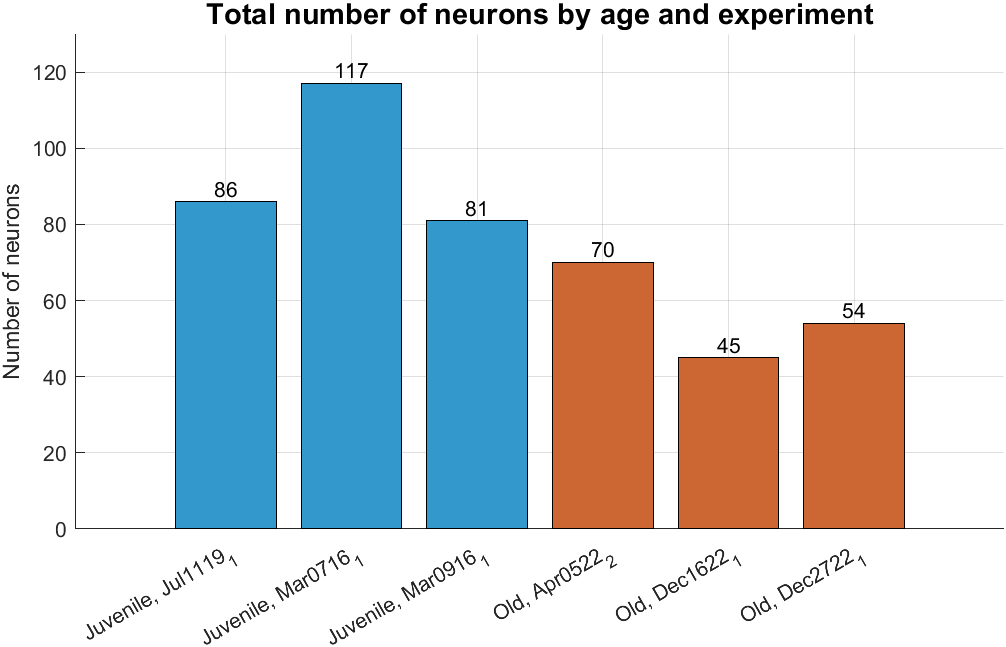
\includegraphics[width=0.8\textwidth]{img/Total_Neurons.png}
    \caption{Total de neuronas por set de datos.}
    \label{total_neurons}
\end{figure}

\begin{figure}
    \centering
    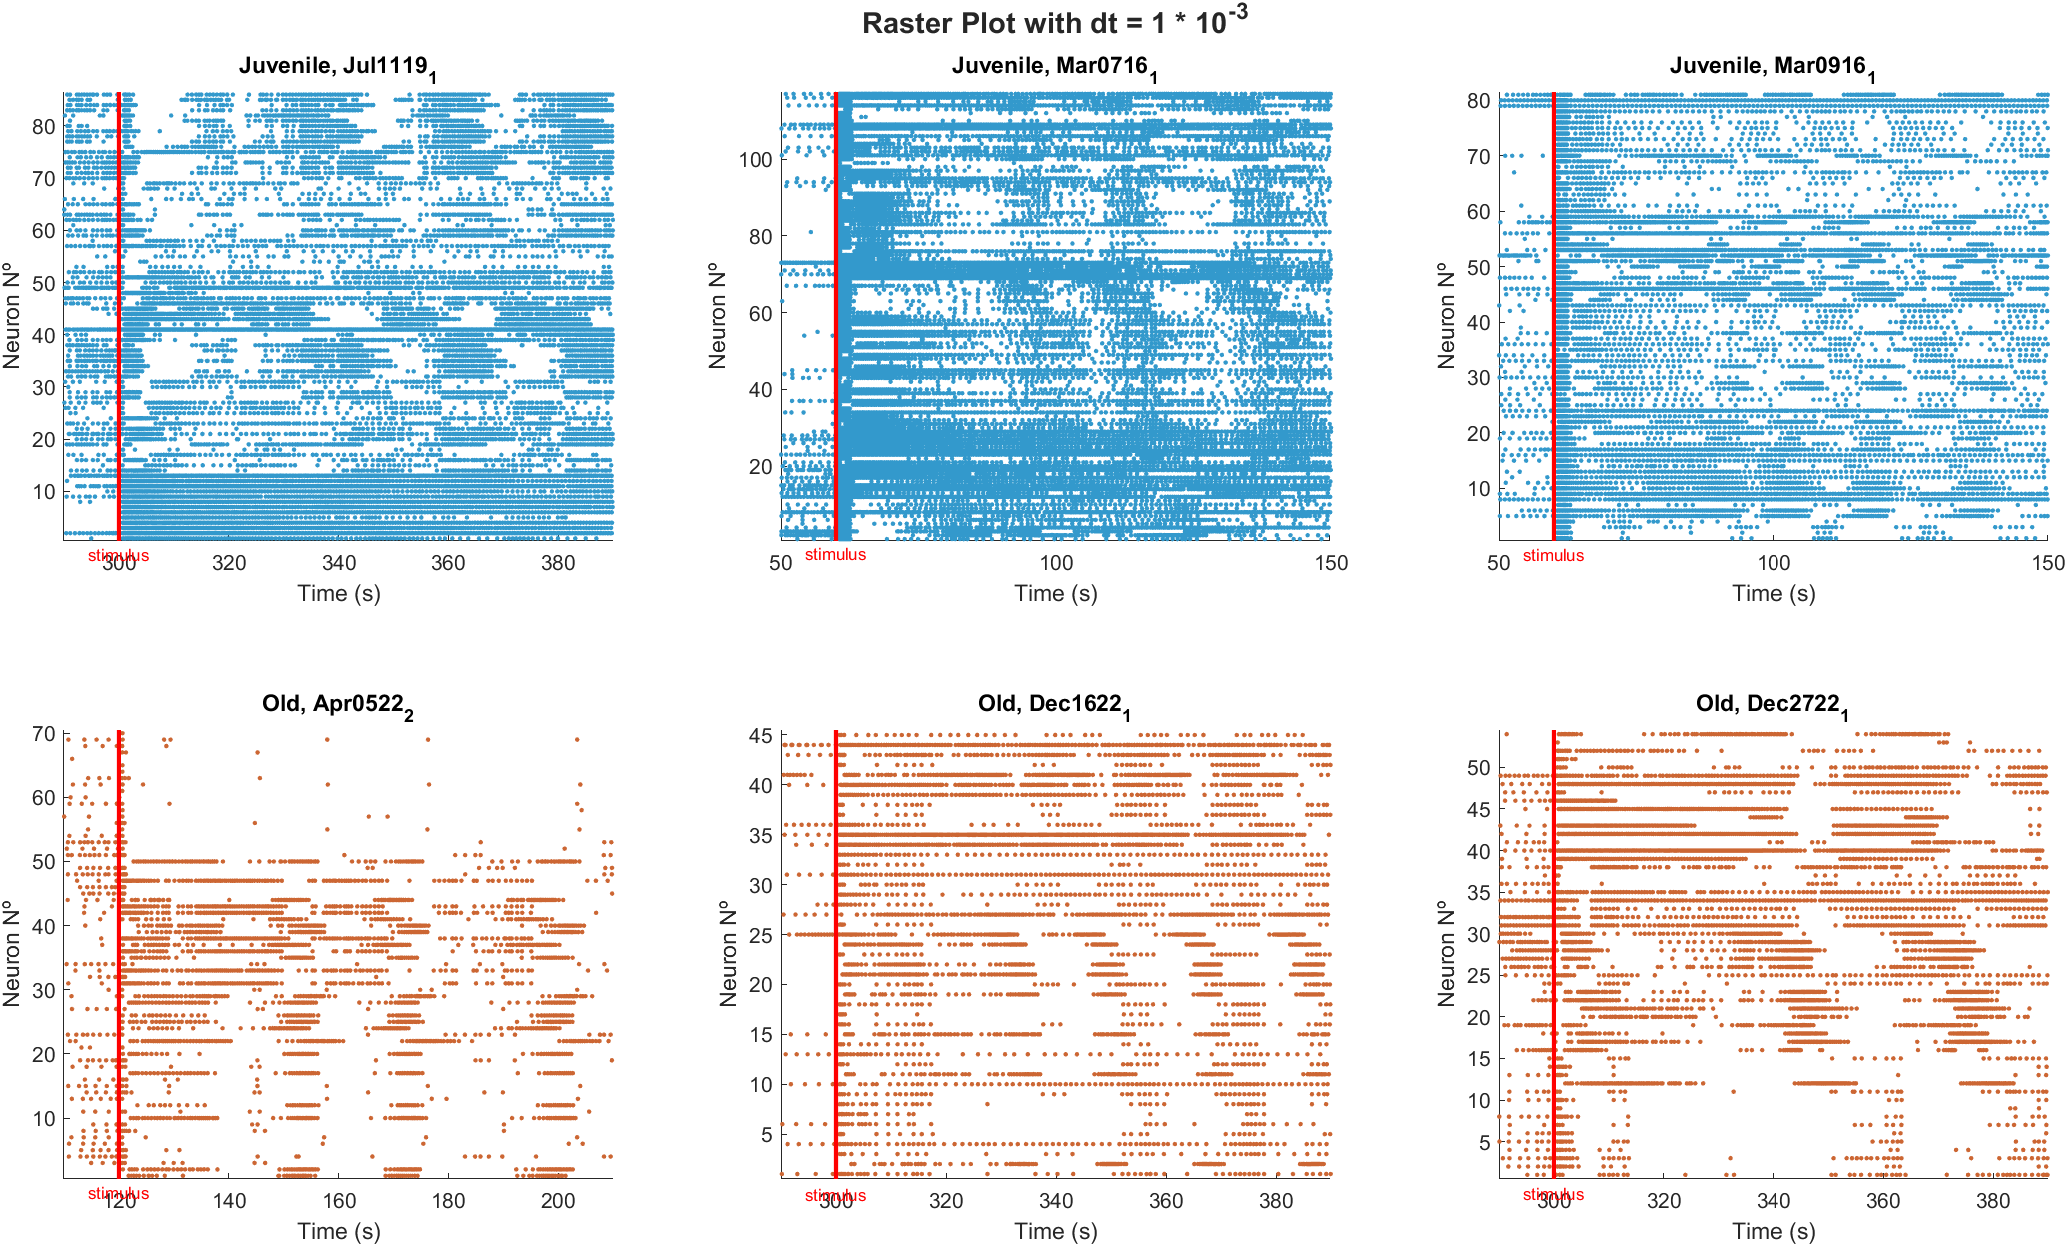
\includegraphics[width=0.9\textwidth]{img/RasterPlot.png}
    \caption{Raster Plot por set de datos.}    
    \label{rasterplot}
\end{figure}

\begin{figure}
    \centering
    \subfloat{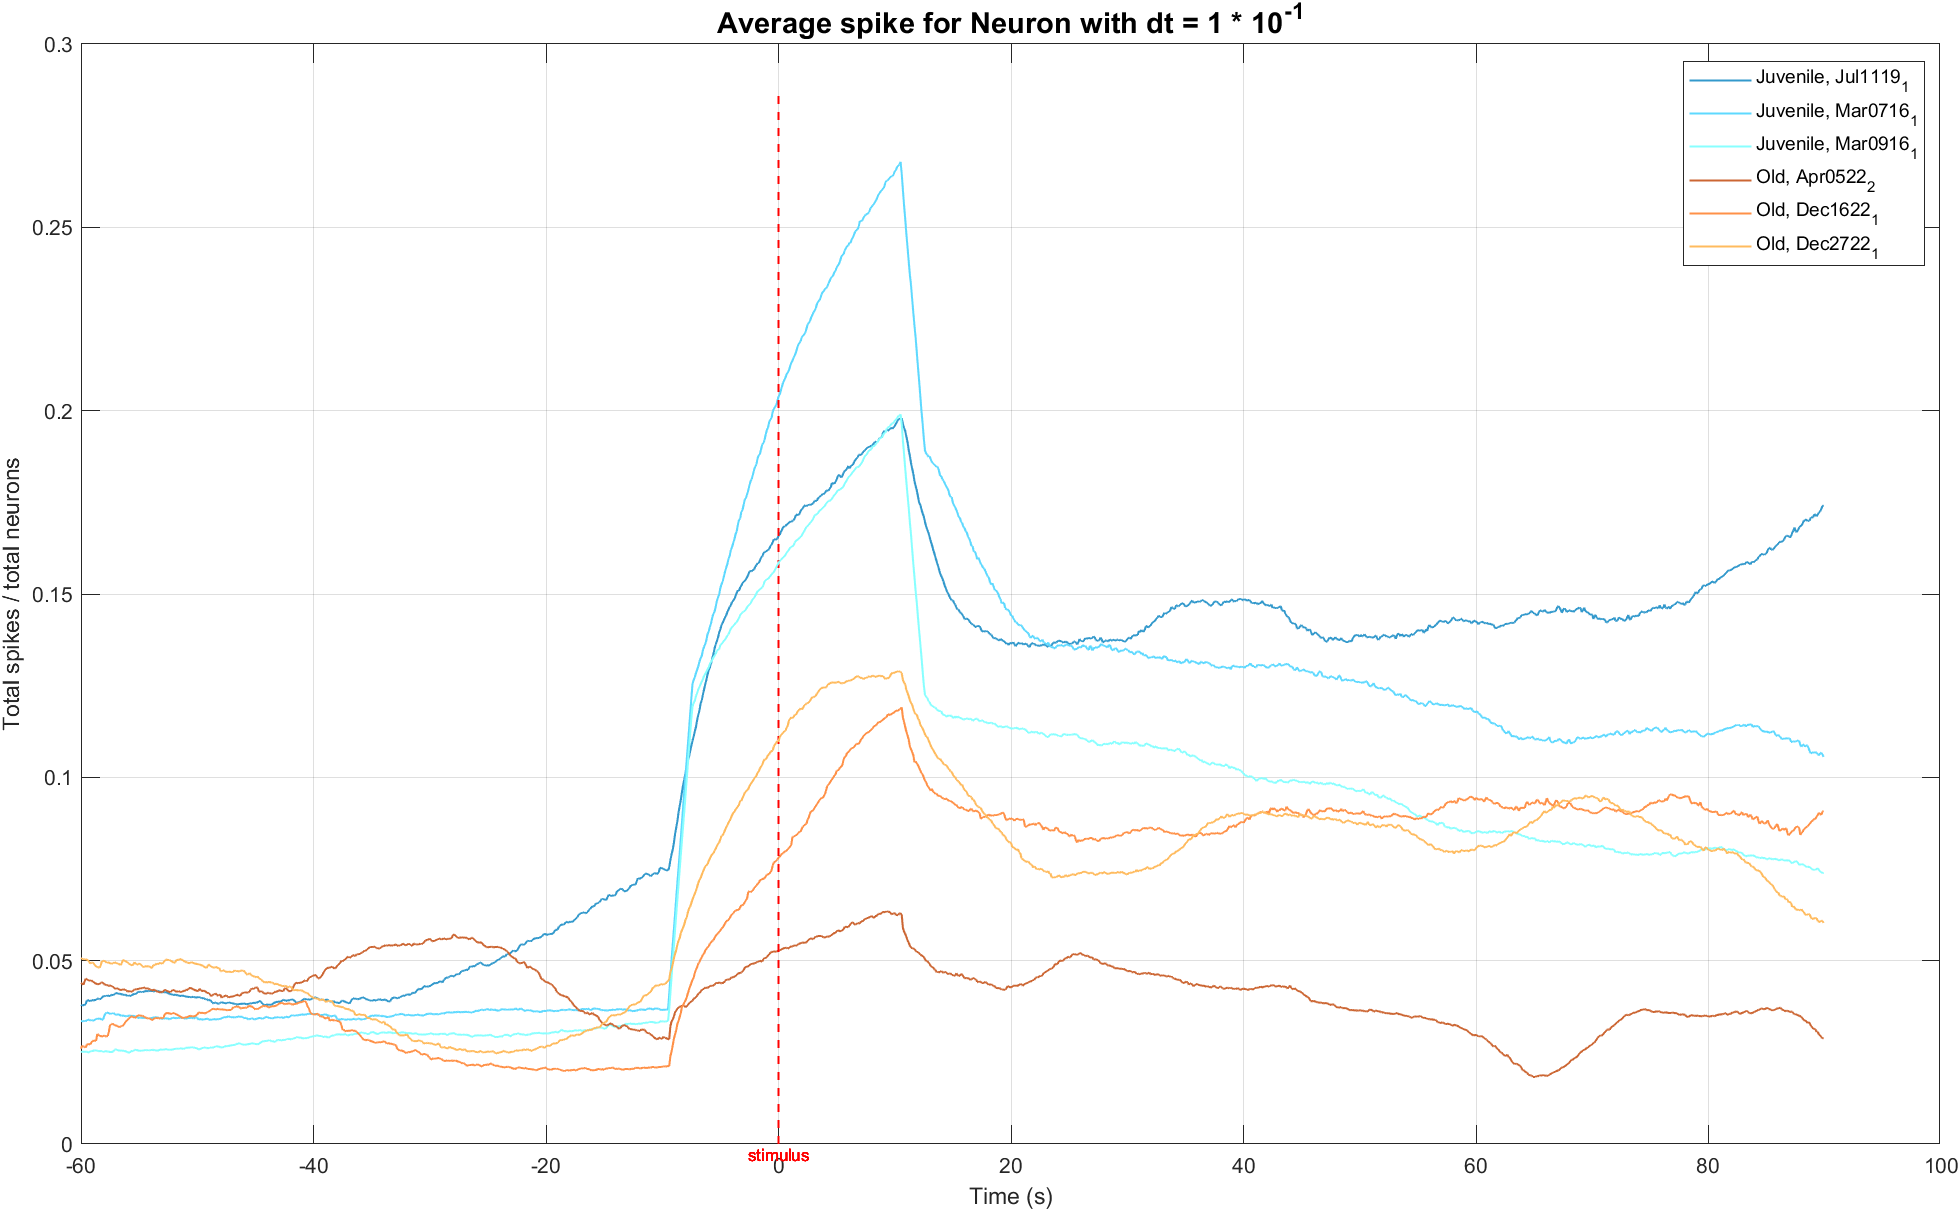
\includegraphics[width=0.8\textwidth]{img/Average_spike_for_Neuron.png}}
    
    \hfill
    
    \subfloat{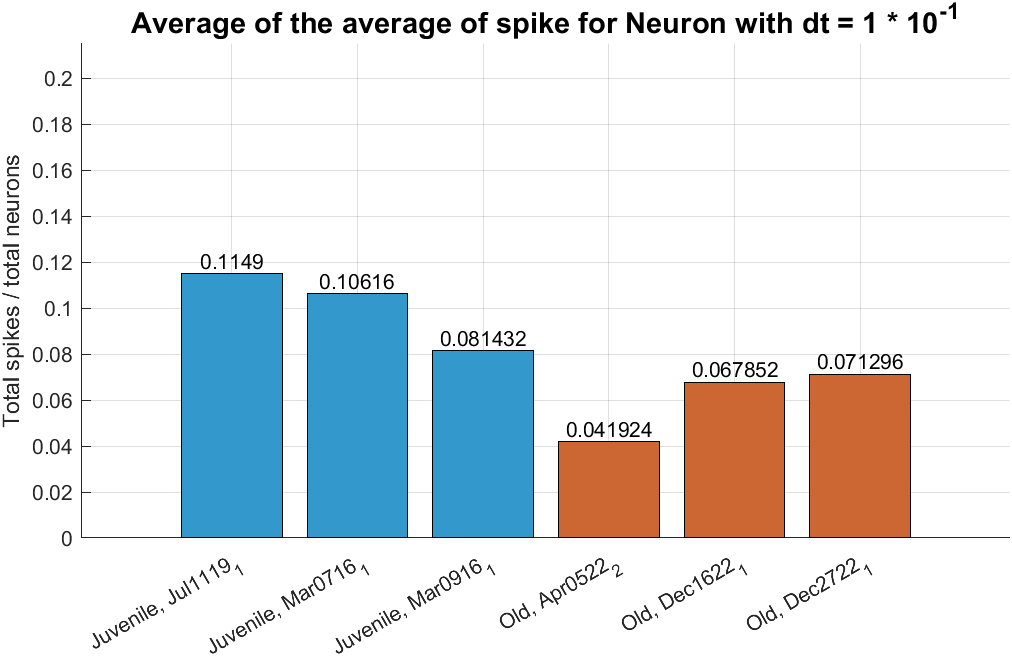
\includegraphics[width=0.8\textwidth]{img/Average_of_the_average_spike_for_Neuron.png}}
    
    \caption{Promedio de spikes totales normalizado por cantidad total de neuronas por set de datos.}
    
    \label{promdelprom}
\end{figure}

\begin{figure}
    \centering
    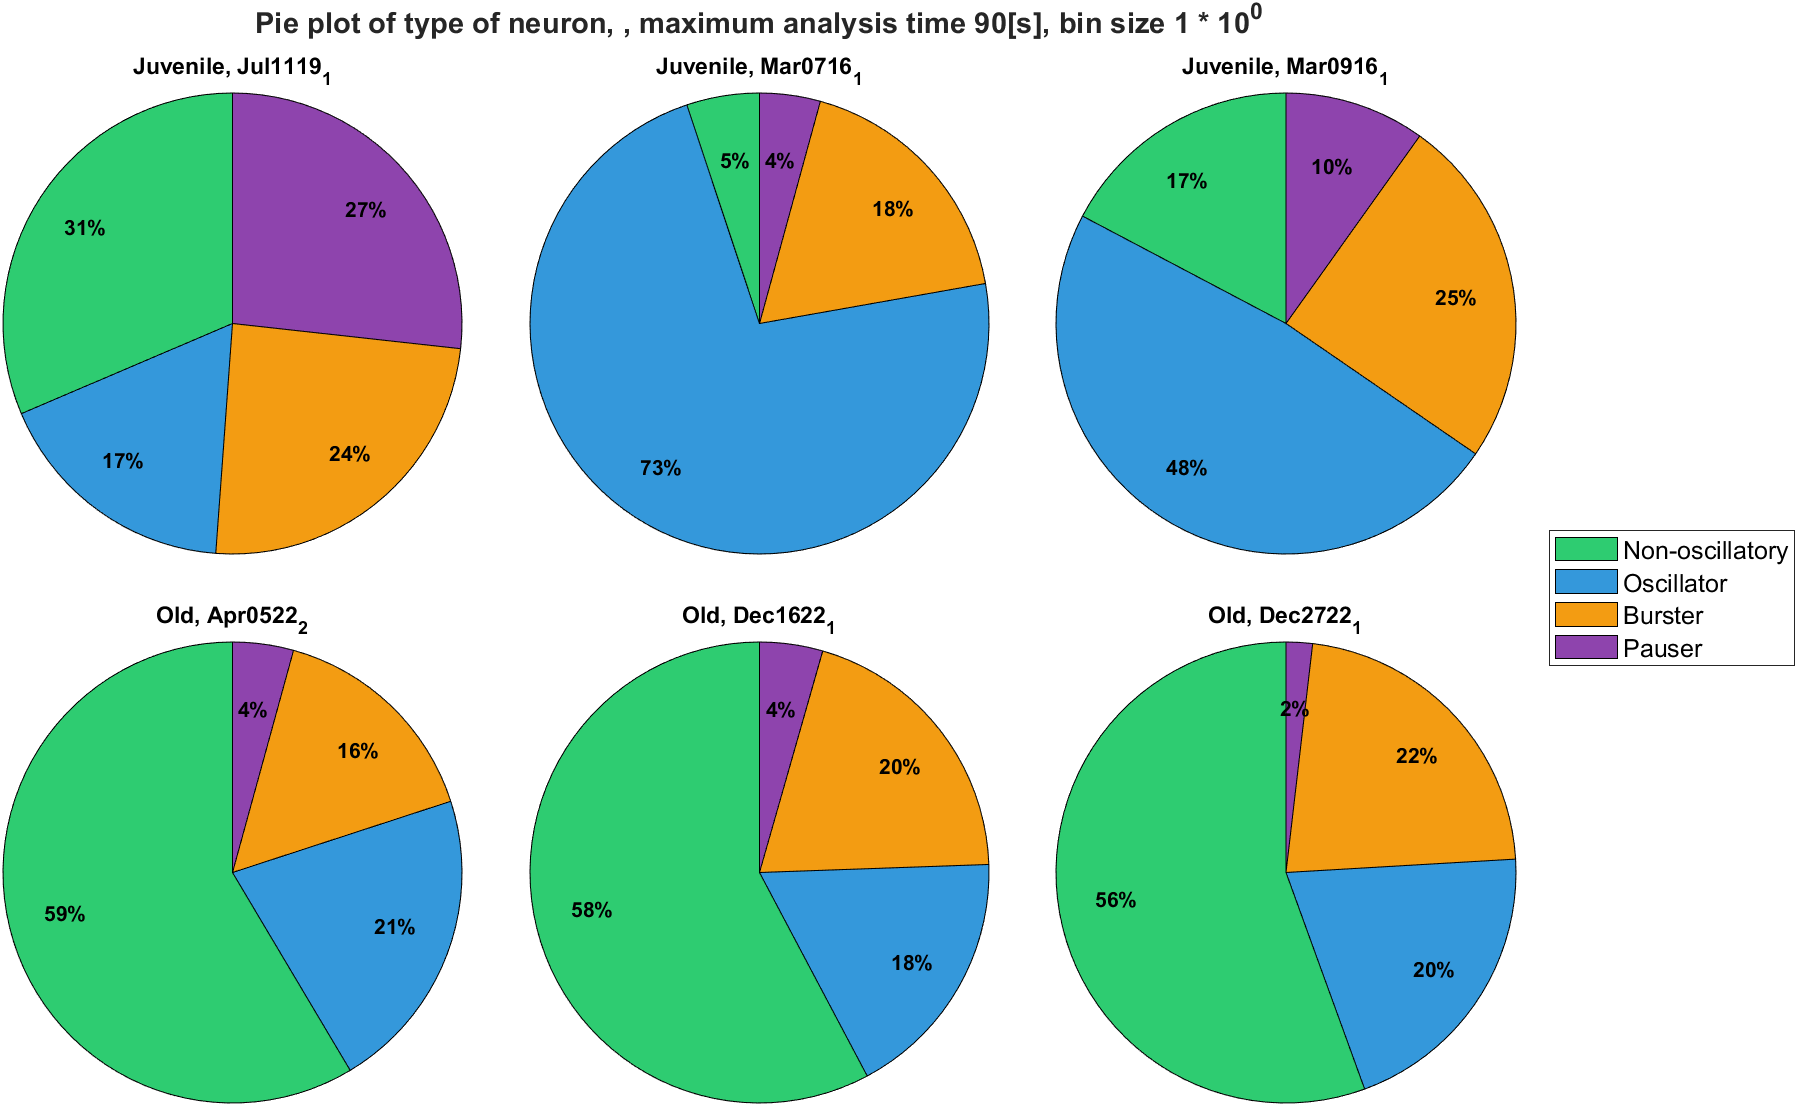
\includegraphics[width=0.8\textwidth]{img/Pie_plot_of_type_of_Neuron.png}
    \caption{Gráfico circular de total de neuronas de cada tipo por set de datos.}    
    \label{pieplot}
\end{figure}

\begin{figure}
    \centering
    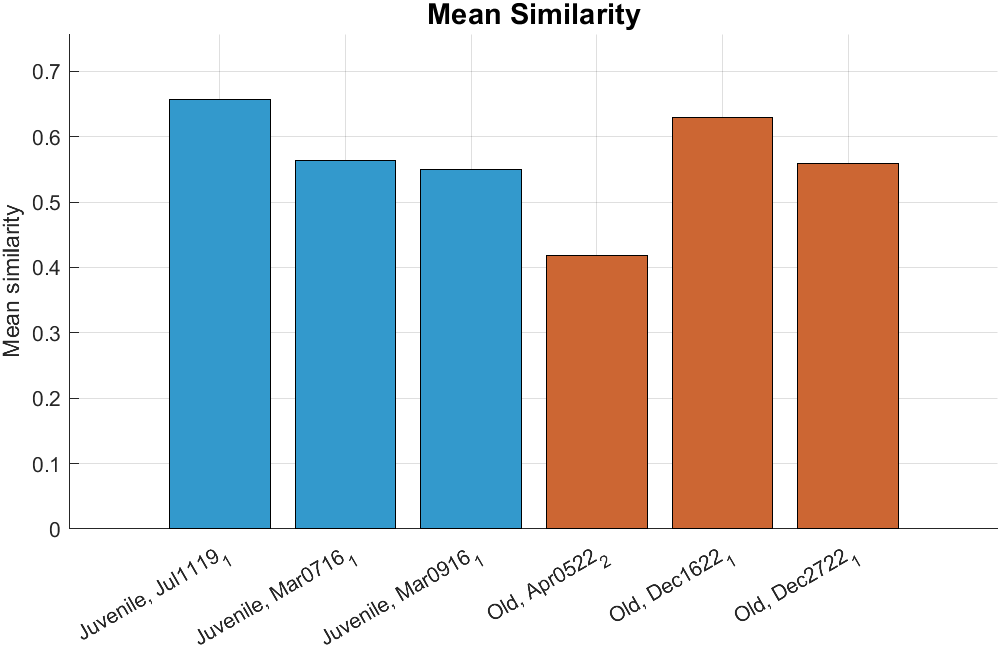
\includegraphics[width=0.8\textwidth]{img/Mean_similarity.png}
    \caption{Promedio de similaridad en matrix de similaridad del coseno por set de datos.}    
    \label{pieplot}
\end{figure}


\begin{figure}
    \centering
    \subfloat{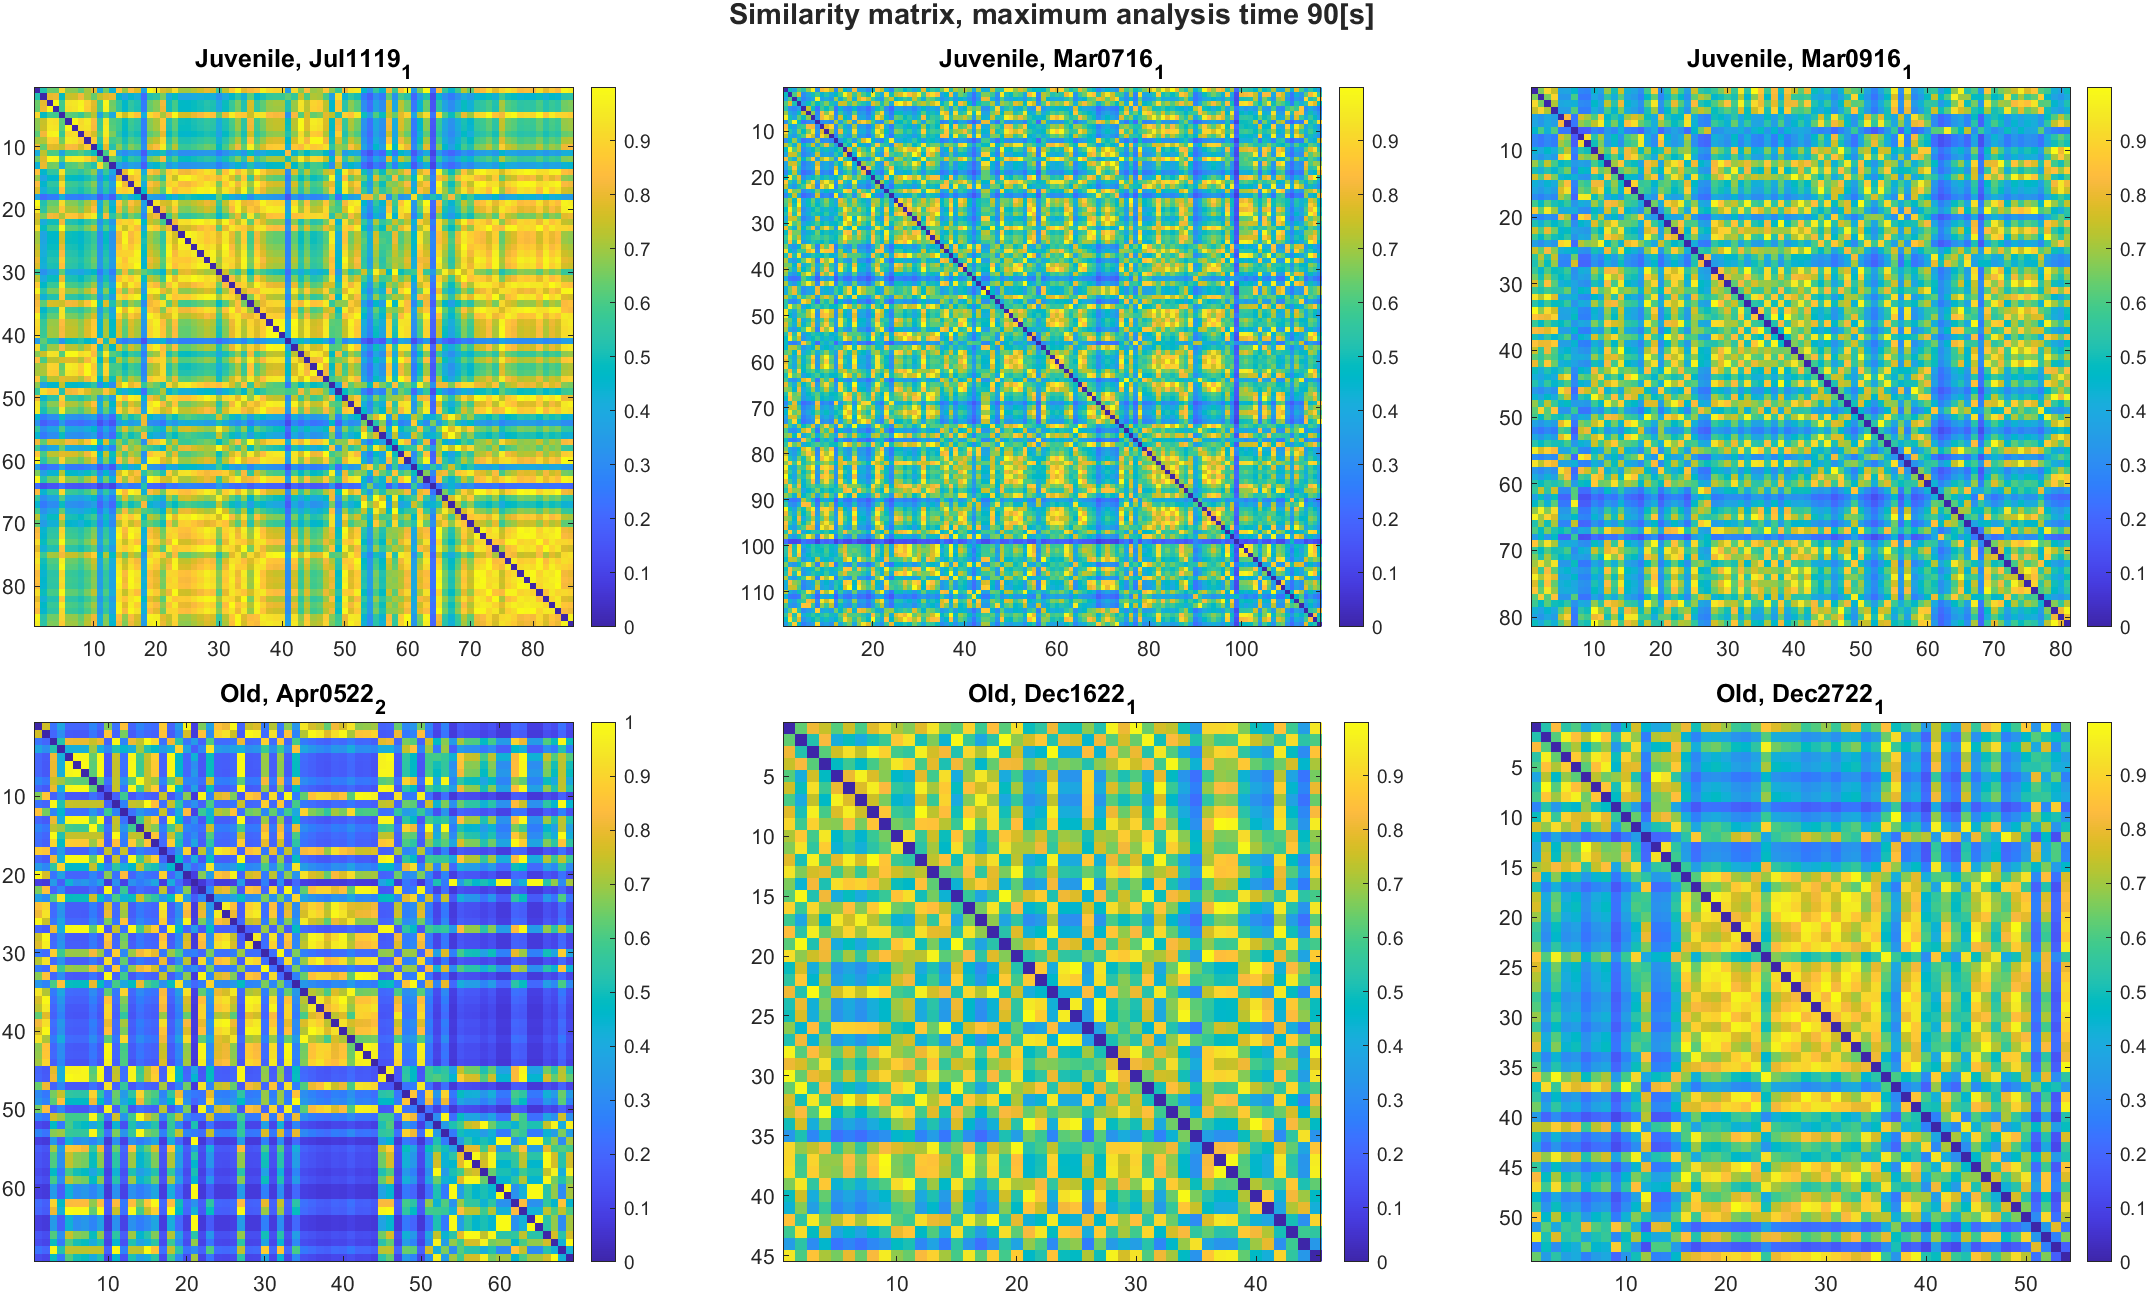
\includegraphics[width=0.8\textwidth]{img/CSM_base.png}}
    
    \hfill
    
    \subfloat{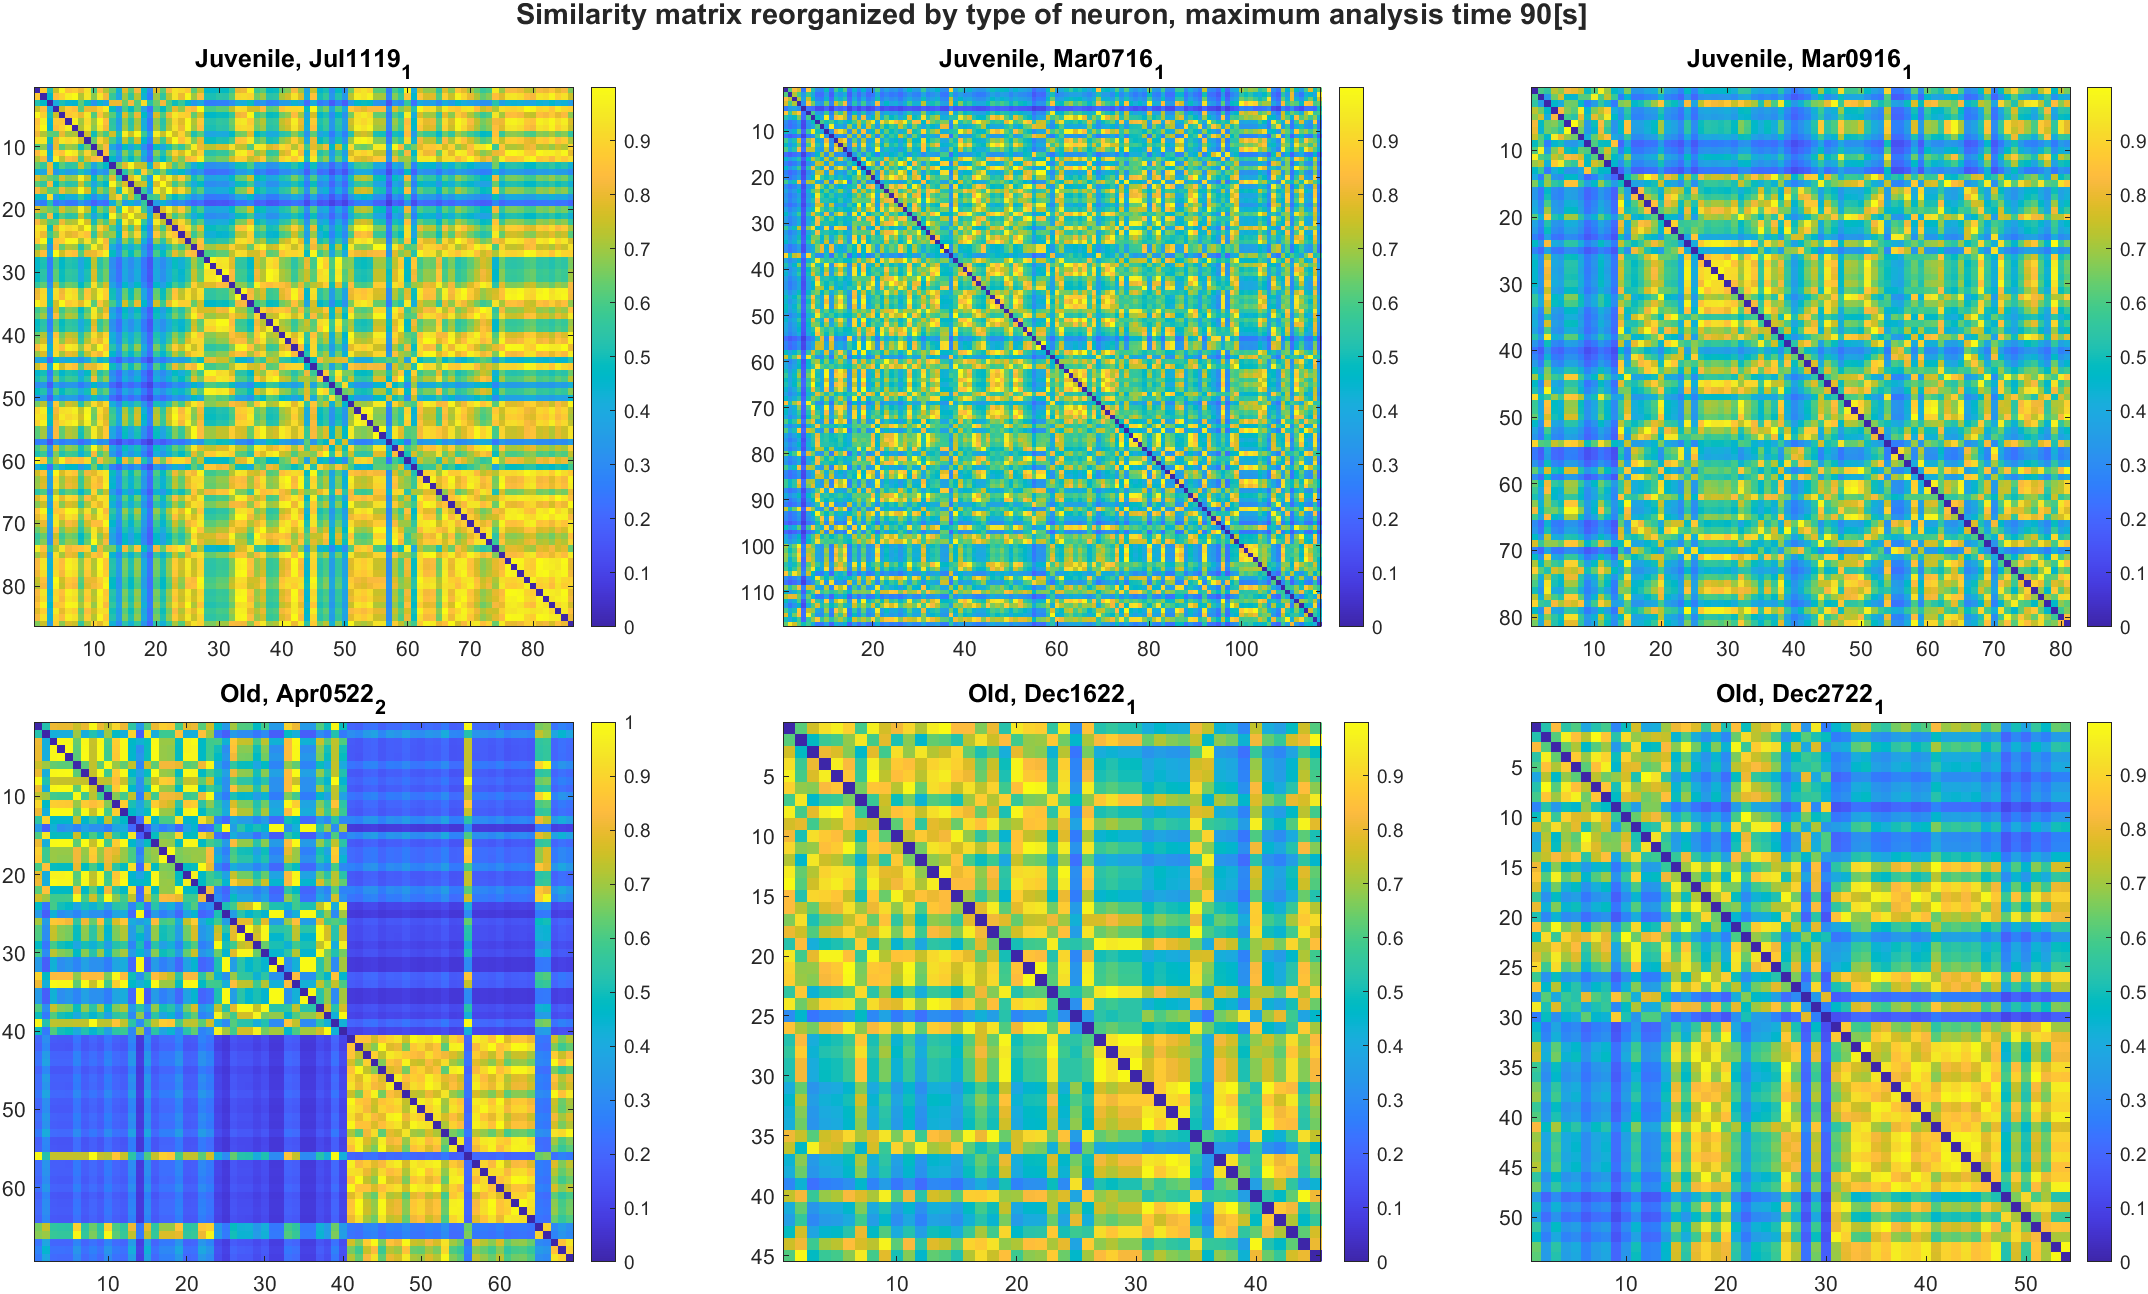
\includegraphics[width=0.8\textwidth]{img/CSM_reorganized.png}}
    
    \caption{Matriz de similaridad del coseno antes y despúes de clasificar las neuronas según patrón de disparo por set de datos.}
    
    \label{csm}
\end{figure}

\begin{figure}
    \centering
    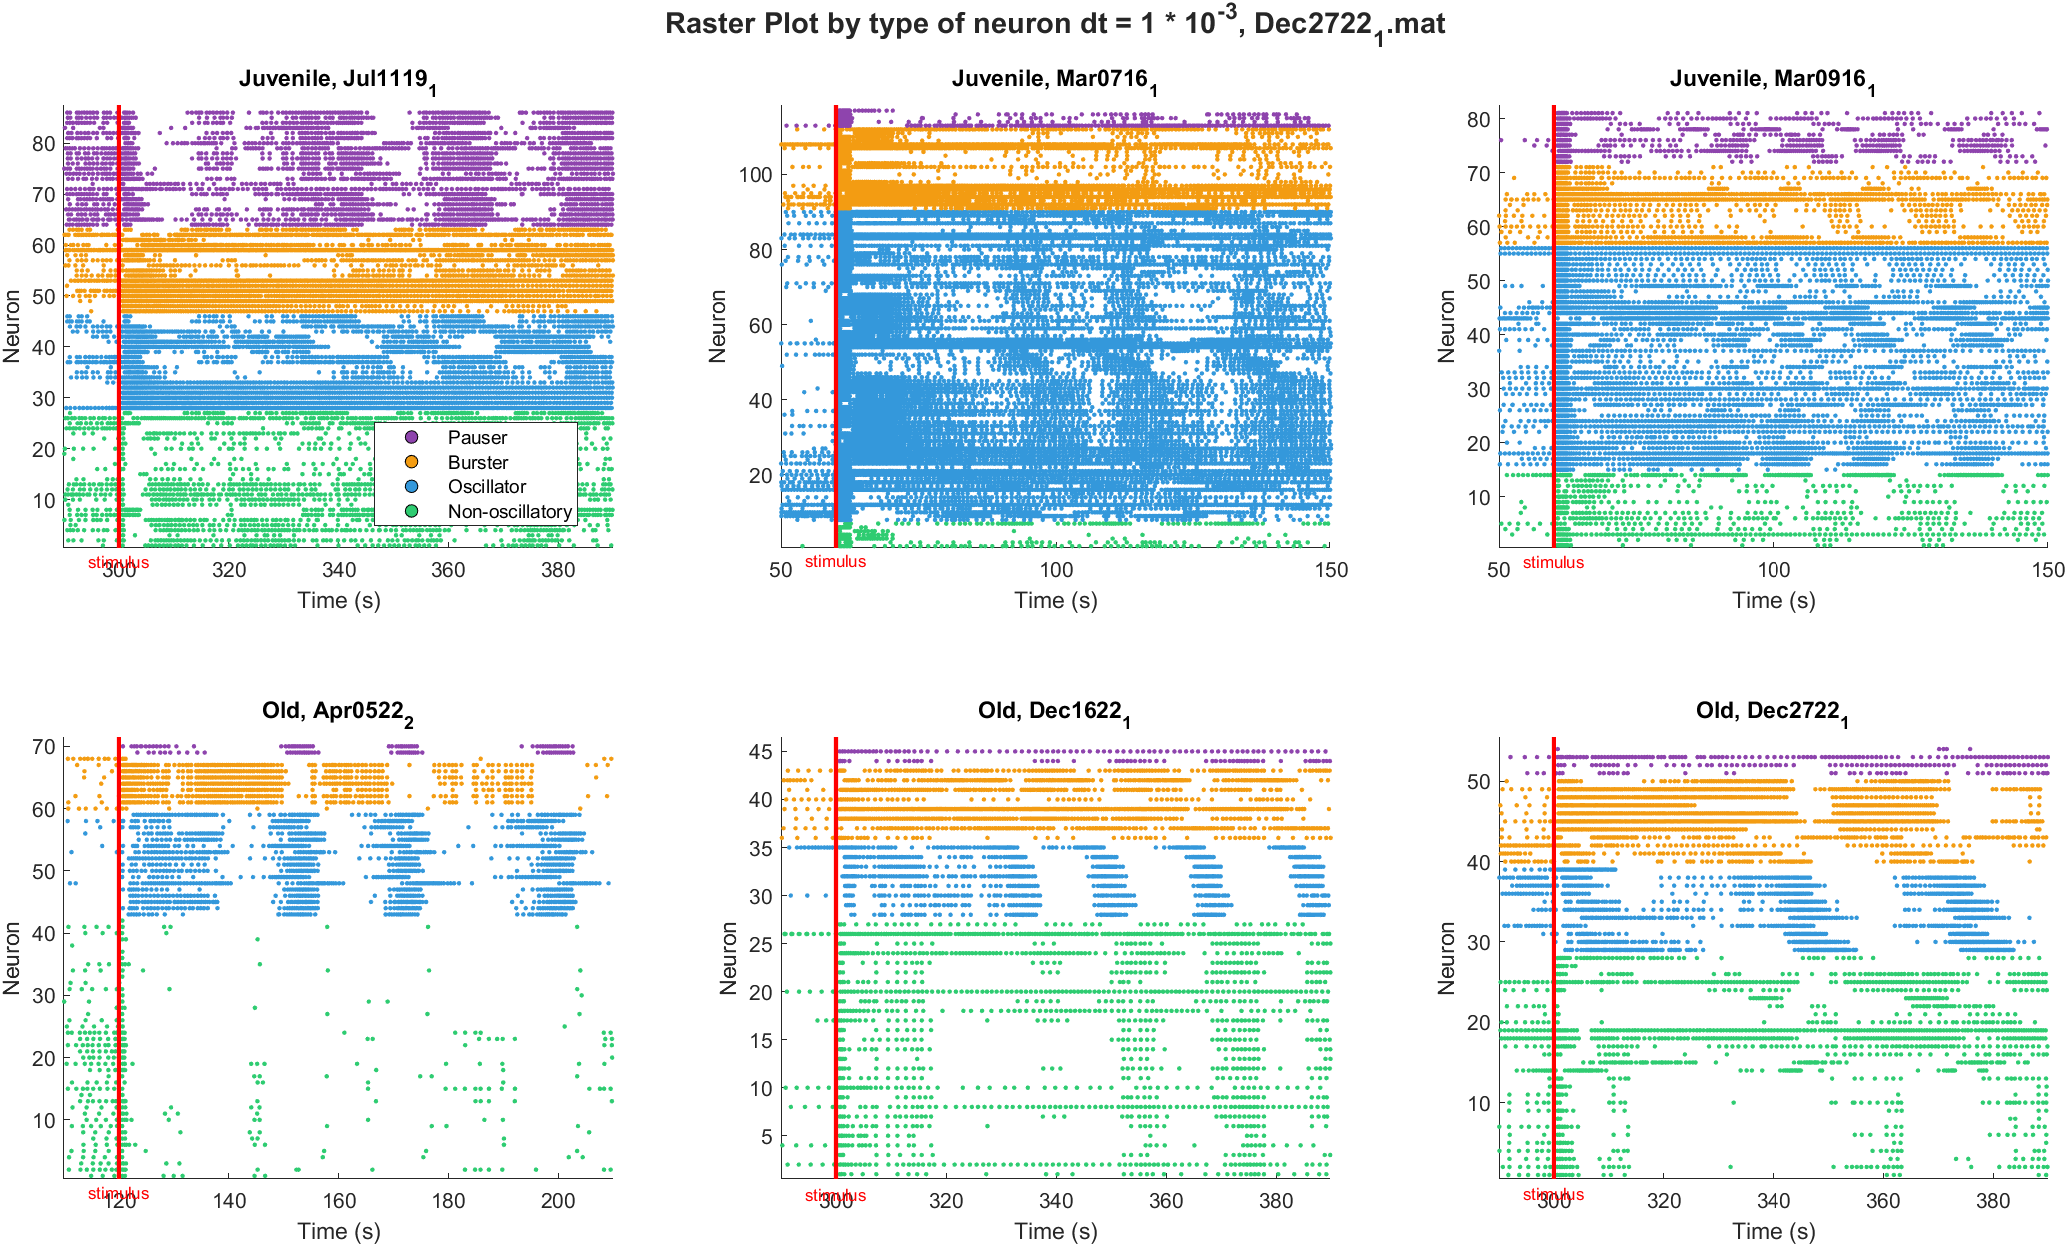
\includegraphics[width=0.7\textwidth]{img/RasterPlot_by_Type.png}
    \caption{Raster Plot con neuronas agrupadas según patrón de oscilación por set de datos.}    
    \label{RP por tipo}
\end{figure}


\begin{figure}
    \centering
    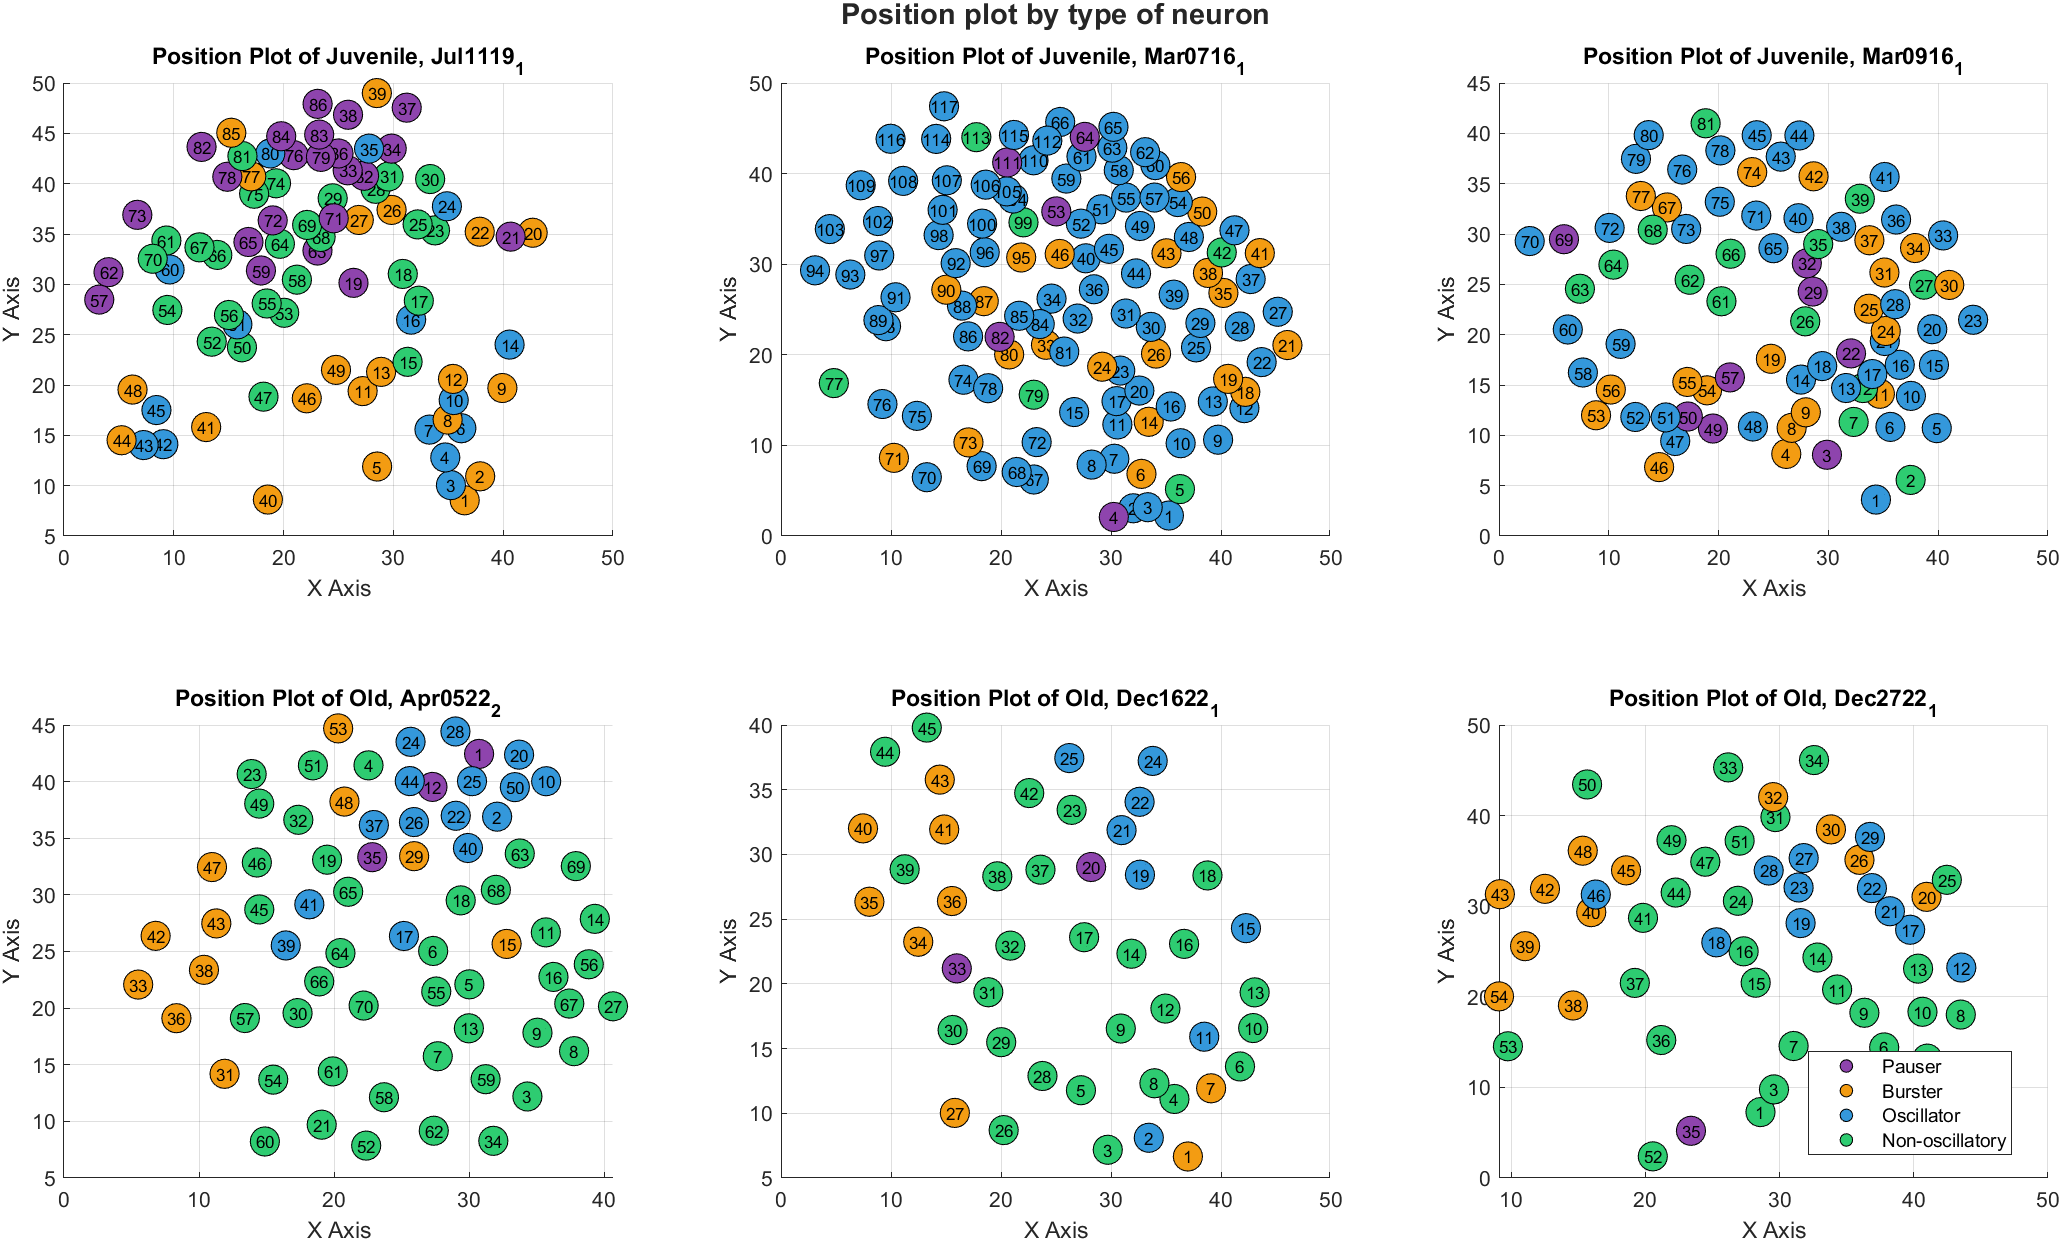
\includegraphics[width=0.7\textwidth]{img/PositionPlot_by_Type.png}
    \caption{Gráfico de posición de neuronas por dataset.}    
    \label{Positionplot}
\end{figure}


Del trabajo realizado se concluye que, al comparar la población joven y envejecida de \textit{Aplysia}, la cantidad total de neuronas disminuye en promedio un 40\%, el promedio de spikes por tiempo, normalizado por el total de neuronas, se reduce en un 50\%, y la cantidad de neuronas oscilatorias disminuye en un 61\%. En este contexto, las neuronas no oscilatorias aumentan, mientras que las demás se mantienen en un rango similar. Finalmente, la posición relativa de los diferentes tipos de neuronas no es concluyente.\\

Todos los códigos utilizados se encuentran en el Github <\url{https://github.com/JavieraRojasM/Practica.git}> .

\clearpage

% \begin{references}


%     \bibitem{bib perdida sinaptica}
%     Etan J. Markus, Ted L. Petit. Neocortical synaptogenesis, aging, and behavior: Lifespan development in the motor-sensory system of the rat. 1987. [en línea] <\url{https://www.sciencedirect.com/science/article/pii/0014488687900458}>

%    \bibitem{bib burst}
%    Ishida, Y., Kozaki, T., Isomura, Y., Ito, S., Isobe, Ki. Age-Dependent Changes in Dopaminergic Neuron Firing Patterns in Substantia Nigra Pars Compacta. 2009. [en línea] <\url{https://link.springer.com/chapter/10.1007/978-3-211-92660-4_10}>

%     \bibitem{bib Ca}
%     Thomas A. Pitler, Philip W. Landfield. Aging-related prolongation of calcium spike duration in rat hippocampal slice neurons. 1990. [en línea]<\url{https://www.sciencedirect.com/science/article/pii/000689939091109T?ref=pdf_download&fr=RR-2&rr=8fc2a2a4af8988a6}>
    
%    \bibitem{bib Potasio}
%     B. Potier, O. Rascol, F. Jazat, Y. Lamour, P. Dutar. Alterations in the properties of hippocampal pyramidal neurons in the aged rat. 1992. [en línea] <\url{https://www.sciencedirect.com/science/article/pii/0306452292902676}>
    
%     \bibitem{bib sensoriales}
%     Kempsell Andrew T. , Fieber Lynne A. Behavioral aging is associated with reduced sensory neuron excitability in Aplysia californica. 2014. [en línea] <\url{https://www.frontiersin.org/journals/aging-neuroscience/articles/10.3389/fnagi.2014.00084/full}>

%    \bibitem{bib cantidad}
%     Bertram Peretz, Malathi Srivatsan. Differences in aging in two neural pathways: Proposed explanations from the nervous system of aplysia. 1992. [en línea] <\url{https://www.sciencedirect.com/science/article/pii/053155659290031T}>
    
%    \bibitem{AMB}
%     Angela M. Bruno, William N. Frost, Mark D. Humphries. Modular Deconstruction Reveals the Dynamical and Physical Building Blocks of a Locomotion Motor Program. 2015. [en línea] <\url{https://www.sciencedirect.com/science/article/pii/S0896627315002019?via%3Dihub}>

% \end{references}
